% =====================================================================
%  Chapitre 1 : Structure d'un projet Django
% =====================================================================
\chapter{Structure d'un projet Django}
\label{ch:structure}

\chapitreresume{Un projet Django est une arborescence de fichiers aux rôles bien
définis. Dans ce chapitre, vous créez le projet \gesibiblio, vous découvrez le rôle
de chaque fichier et vous configurez les réglages essentiels, notamment le fichier
\code{settings.py}. Vous lancez aussi le serveur de développement pour la première
fois.}

\begin{objectifs}
\begin{itemize}
  \item Créer un projet Django avec \code{django-admin startproject}.
  \item Lire et expliquer l'arborescence d'un projet.
  \item Décrire le rôle de \code{manage.py}, \code{settings.py}, \code{urls.py},
        \code{wsgi.py} et \code{asgi.py}.
  \item Comprendre les principaux réglages de \code{settings.py}.
  \item Lancer le serveur de développement et appliquer les migrations initiales.
  \item Mettre en place les fichiers de base d'un projet propre : dépendances,
        variables d'environnement et versionnement.
\end{itemize}
\end{objectifs}

\section{Créer le projet}

Placez-vous dans le dossier de travail créé au chapitre précédent, puis lancez la
commande suivante :

\begin{terminal}
django-admin startproject gesibiblio .
\end{terminal}

Le point final est important. Il demande à Django de créer le projet
\emph{dans le dossier courant}, et non dans un sous-dossier supplémentaire.

\begin{attention}
Si vous oubliez le point, Django crée un dossier \code{gesibiblio/} qui contient
lui-même un dossier \code{gesibiblio/}. Vous obtenez une arborescence imbriquée du
type \code{gesibiblio/gesibiblio/settings.py}. Ce n'est pas faux, mais cela
complique les chemins et les commandes. Pour ce module, utilisez le point.
\end{attention}

Vérifiez le résultat :

\begin{terminal}
dir
\end{terminal}

Sous macOS ou Linux, utilisez \code{ls -la}. Vous devez voir un fichier
\code{manage.py} et un dossier \code{gesibiblio/}.

\section{L'arborescence du projet}

\begin{figure}[htbp]
\centering
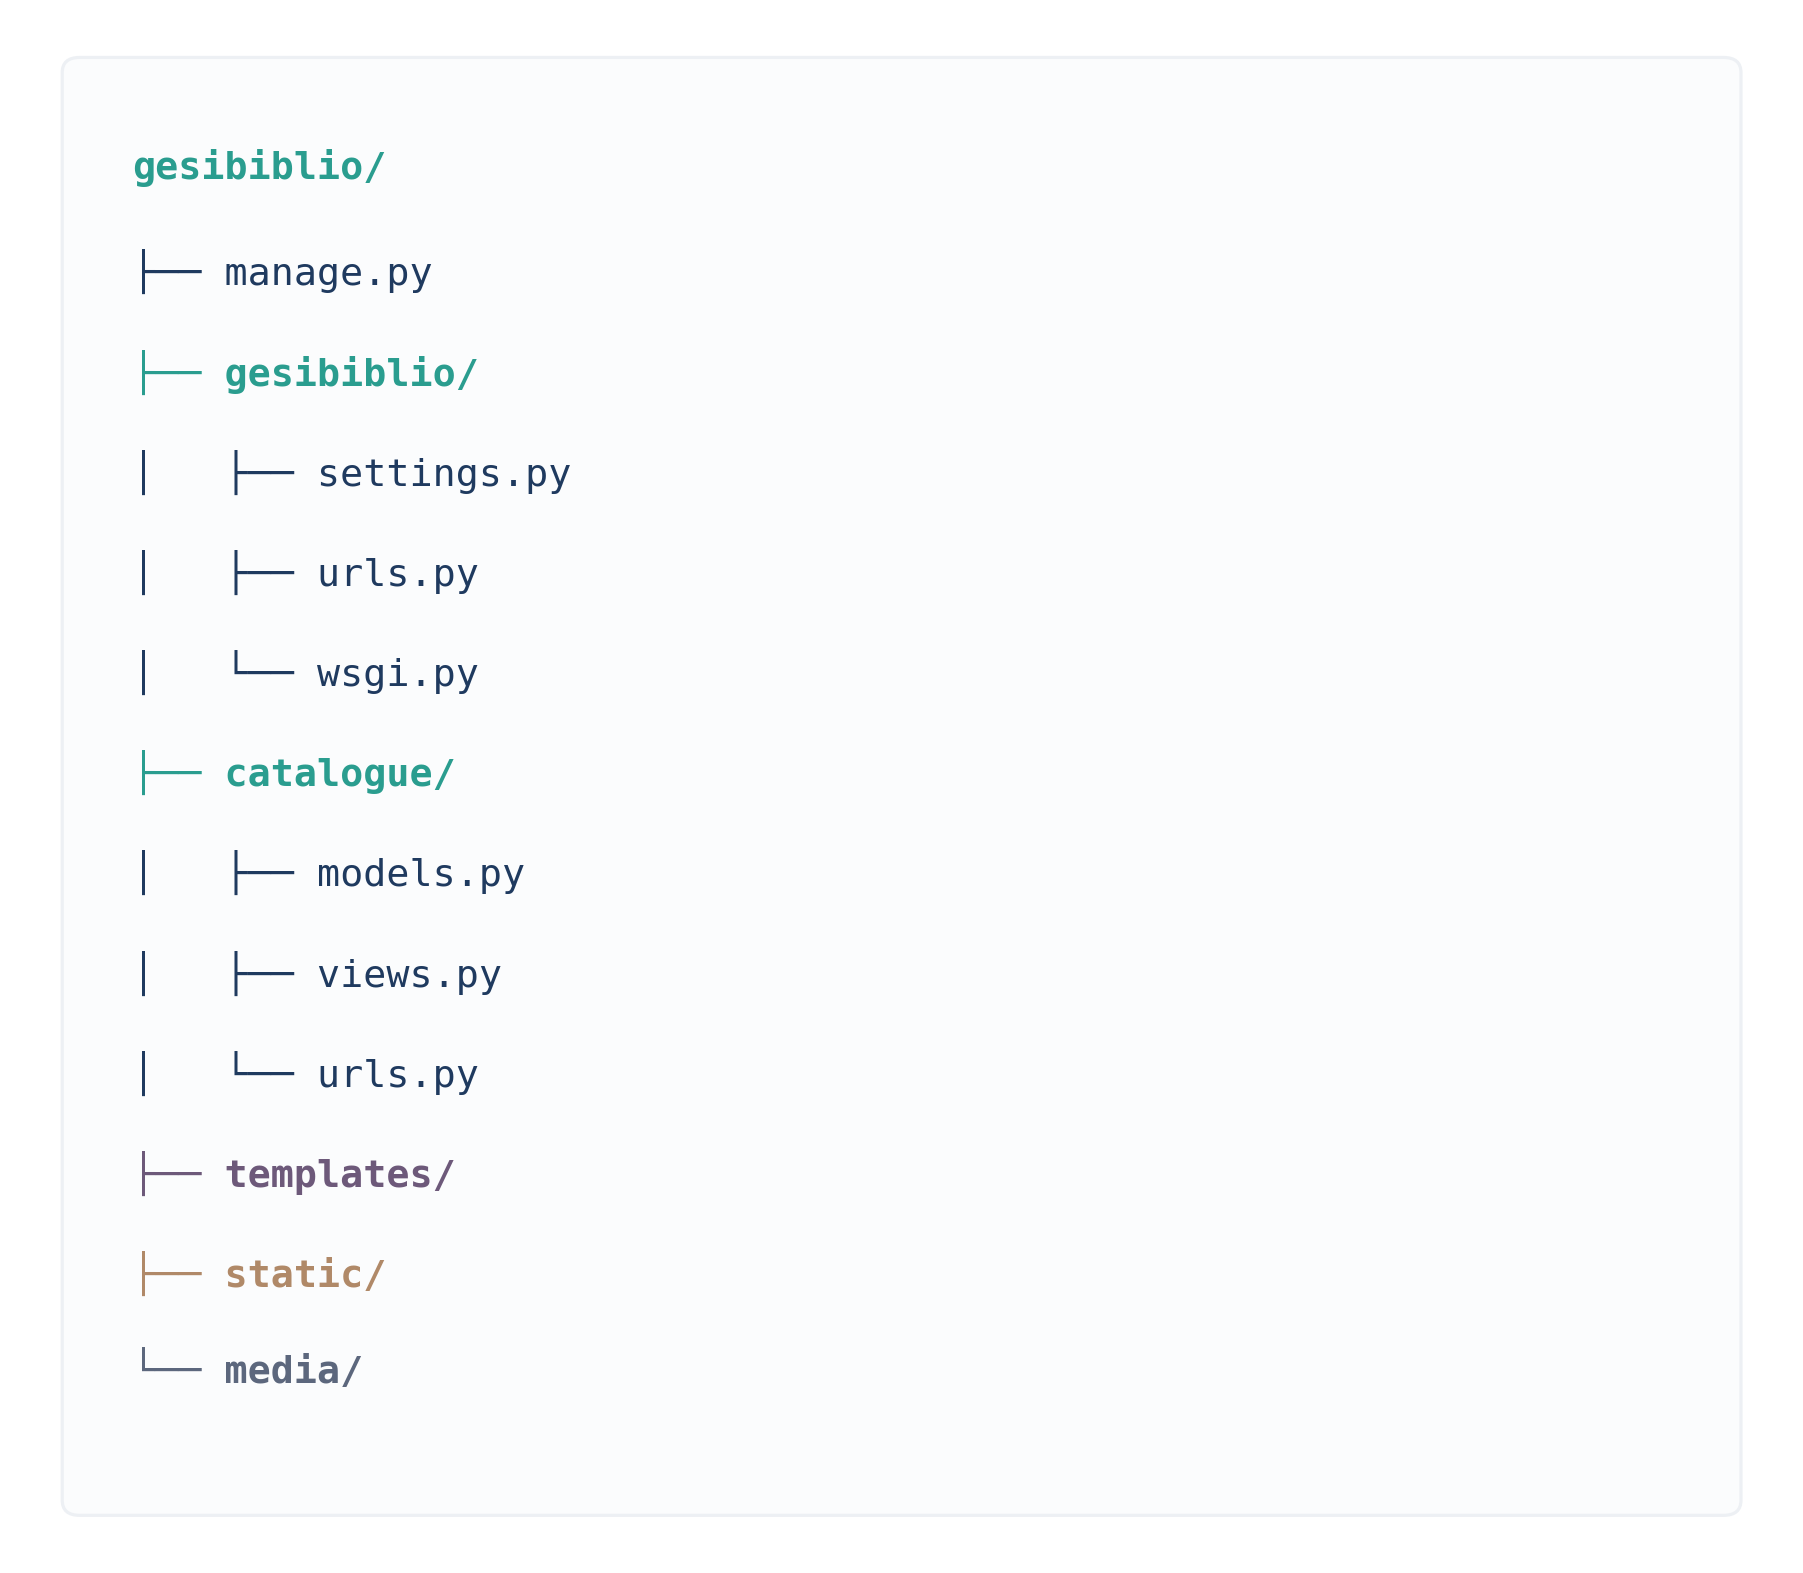
\includegraphics[width=0.72\textwidth]{images/arborescence.png}
\caption{Les dossiers et fichiers principaux d'un projet Django. Les dossiers sont
en couleur, les fichiers Python en bleu foncé.}
\label{fig:arborescence}
\end{figure}

Voici l'arborescence complète après la création du projet :

\begin{codebox}[tree]{Arborescence initiale}
gesibiblio/
|-- manage.py
|-- db.sqlite3
`-- gesibiblio/
    |-- __init__.py
    |-- __pycache__/
    |-- asgi.py
    |-- settings.py
    |-- urls.py
    `-- wsgi.py
\end{codebox}

Le fichier \code{db.sqlite3} n'apparaît qu'après la première migration. Le dossier
\code{\_\_pycache\_\_} est créé automatiquement par Python : il contient la version
compilée des modules. Il ne doit jamais être versionné.

\begin{note}
Le nom \code{gesibiblio} est utilisé à deux niveaux : le dossier du projet et le
paquet Python de configuration. C'est une convention courante. Le nom du projet
doit être un identifiant Python valide : lettres minuscules, chiffres et tirets du
bas, sans espace ni accent.
\end{note}

\section{Le rôle de chaque fichier}

\begin{table}[htbp]
\centering
\small
\begin{tabularx}{\textwidth}{L{4.1cm} X C{2.1cm}}
\toprule
\textbf{Fichier ou dossier} & \textbf{Rôle} & \textbf{À modifier ?} \\
\midrule
\code{manage.py} & Point d'entrée des commandes du projet. Il appelle
\code{django-admin} avec le bon fichier de réglages. & Rarement \\
\code{gesibiblio/\_\_init\_\_.py} & Indique que le dossier est un paquet Python.
Il reste vide. & Non \\
\code{gesibiblio/settings.py} & Configuration complète : applications, base de
données, gabarits, langue, fichiers statiques, sécurité. & Oui, très souvent \\
\code{gesibiblio/urls.py} & Table de routage racine. Elle associe les URL aux vues
et inclut les URL des applications. & Oui \\
\code{gesibiblio/asgi.py} & Point d'entrée ASGI, pour les serveurs asynchrones.
Utile en production. & Non, en général \\
\code{gesibiblio/wsgi.py} & Point d'entrée WSGI, pour les serveurs synchrones
classiques comme Gunicorn. & Non, en général \\
\code{db.sqlite3} & Base de données SQLite créée par les migrations. & Non, généré \\
\code{migrations/} & Historique des modifications du schéma de base. & Non, généré \\
\code{\_\_pycache\_\_/} & Cache des fichiers Python compilés. & Non, généré \\
\bottomrule
\end{tabularx}
\caption{Rôle des fichiers créés par \code{startproject}.}
\end{table}

\subsection{manage.py}

\code{manage.py} est le couteau suisse du projet. Il permet de lancer le serveur,
de créer les migrations, de les appliquer, d'ouvrir un shell Python, de créer un
superutilisateur, etc.

\begin{codebox}[python]{manage.py}
#!/usr/bin/env python
"""Django's command-line utility for administrative tasks."""
import os
import sys


def main():
    """Run administrative tasks."""
    os.environ.setdefault("DJANGO_SETTINGS_MODULE", "gesibiblio.settings")
    try:
        from django.core.management import execute_from_command_line
    except ImportError as exc:
        raise ImportError(
            "Couldn't import Django. Are you sure it's installed and "
            "available on your PYTHONPATH environment variable? Did you "
            "forget to activate a virtual environment?"
        ) from exc
    execute_from_command_line(sys.argv)


if __name__ == "__main__":
    main()
\end{codebox}

La ligne essentielle appelle \code{os.environ.setdefault} avec le nom du module
de réglages, \code{gesibiblio.settings}. Elle indique à Django quel fichier de
configuration utiliser. C'est pour cela que toutes les commandes commencent par
\code{python manage.py} : le script transmet le bon contexte à Django.

\begin{bonne}
Utilisez toujours \code{python manage.py} plutôt que \code{django-admin} lorsque
vous êtes dans le projet. Vous êtes ainsi certain que la bonne configuration et le
bon environnement virtuel sont utilisés.
\end{bonne}

\subsection{settings.py, le centre de configuration}

\code{settings.py} est le fichier le plus important du projet. Il contient des
variables Python en majuscules, lues par Django au démarrage. Une erreur dans ce
fichier peut empêcher tout le site de démarrer.

Voici le fichier généré, avec des commentaires en français et deux adaptations :
la langue et le fuseau horaire.

\begin{codebox}[python]{gesibiblio/settings.py}
"""
Réglages Django pour le projet GesiBiblio.

Ce fichier contient la configuration globale du site.
Pour la documentation complète, voir :
https://docs.djangoproject.com/fr/5.2/topics/settings/
"""
from pathlib import Path

# Chemin absolu du dossier qui contient manage.py.
# BASE_DIR sert à construire tous les autres chemins du projet.
BASE_DIR = Path(__file__).resolve().parent.parent

# Clé secrète utilisée pour signer les sessions et les jetons CSRF.
# En production, elle doit venir d'une variable d'environnement.
SECRET_KEY = "django-insecure-remplacez-cette-cle-en-production"

# Mode debug : affiche les erreurs détaillées. À désactiver en production.
DEBUG = True

# Liste des noms de domaine autorisés. Vide accepte localhost en développement.
ALLOWED_HOSTS = []

# Applications installées dans le projet.
INSTALLED_APPS = [
    "django.contrib.admin",
    "django.contrib.auth",
    "django.contrib.contenttypes",
    "django.contrib.sessions",
    "django.contrib.messages",
    "django.contrib.staticfiles",
]

# Chaîne de middlewares exécutés à chaque requête et à chaque réponse.
MIDDLEWARE = [
    "django.middleware.security.SecurityMiddleware",
    "django.contrib.sessions.middleware.SessionMiddleware",
    "django.middleware.common.CommonMiddleware",
    "django.middleware.csrf.CsrfViewMiddleware",
    "django.contrib.auth.middleware.AuthenticationMiddleware",
    "django.contrib.messages.middleware.MessageMiddleware",
    "django.middleware.clickjacking.XFrameOptionsMiddleware",
]

# Module Python qui contient la table de routage racine.
ROOT_URLCONF = "gesibiblio.urls"

# Configuration du moteur de gabarits.
TEMPLATES = [
    {
        "BACKEND": "django.template.backends.django.DjangoTemplates",
        "DIRS": [],
        "APP_DIRS": True,
        "OPTIONS": {
            "context_processors": [
                "django.template.context_processors.debug",
                "django.template.context_processors.request",
                "django.contrib.auth.context_processors.auth",
                "django.contrib.messages.context_processors.messages",
            ],
        },
    },
]

# Point d'entrée WSGI utilisé par les serveurs de production.
WSGI_APPLICATION = "gesibiblio.wsgi.application"

# Base de données. SQLite est parfait pour apprendre et pour un petit site.
DATABASES = {
    "default": {
        "ENGINE": "django.db.backends.sqlite3",
        "NAME": BASE_DIR / "db.sqlite3",
    }
}

# Règles de validation des mots de passe.
AUTH_PASSWORD_VALIDATORS = [
    {
        "NAME": "django.contrib.auth.password_validation."
                "UserAttributeSimilarityValidator"
    },
    {
        "NAME": "django.contrib.auth.password_validation."
                "MinimumLengthValidator"
    },
    {
        "NAME": "django.contrib.auth.password_validation."
                "CommonPasswordValidator"
    },
    {
        "NAME": "django.contrib.auth.password_validation."
                "NumericPasswordValidator"
    },
]

# Langue de l'interface et format des dates.
LANGUAGE_CODE = "fr-fr"

# Fuseau horaire du projet. Adaptez-le à votre pays.
TIME_ZONE = "Africa/Porto-Novo"

USE_I18N = True
USE_TZ = True

# URL de base des fichiers statiques (CSS, JavaScript, images).
STATIC_URL = "static/"

# Type de clé primaire par défaut des modèles.
DEFAULT_AUTO_FIELD = "django.db.models.BigAutoField"
\end{codebox}

\begin{note}
La valeur de \code{SECRET\_KEY} générée par Django est unique et aléatoire. Celle
ci-dessus est un exemple. Ne la publiez jamais et ne la mettez jamais dans un
dépôt Git public. Le chapitre suivant montre comment la déplacer dans une variable
d'environnement.
\end{note}

\subsection{Les réglages essentiels expliqués}

\begin{table}[htbp]
\centering
\small
\begin{tabularx}{\textwidth}{L{4.2cm} X}
\toprule
\textbf{Réglage} & \textbf{Explication} \\
\midrule
\code{BASE\_DIR} & Chemin absolu du dossier du projet. Il permet d'écrire des
chemins portables, par exemple \code{BASE\_DIR / "templates"}. \\
\code{SECRET\_KEY} & Clé de signature cryptographique. Elle protège les sessions,
les cookies et les formulaires. Elle doit rester secrète. \\
\code{DEBUG} & En mode \code{True}, Django affiche les erreurs détaillées et sert
les fichiers statiques. En production, il faut la mettre à \code{False}. \\
\code{ALLOWED\_HOSTS} & Liste des domaines autorisés à servir le site. En
développement, \code{localhost} et \code{127.0.0.1} suffisent. \\
\code{INSTALLED\_APPS} & Liste des applications actives. Chaque application ajoutée
au projet doit y figurer. \\
\code{MIDDLEWARE} & Couches qui traitent la requête et la réponse : sécurité,
sessions, authentification, messages, protection CSRF. \\
\code{ROOT\_URLCONF} & Module de routage principal. Il pointe vers
\code{gesibiblio/urls.py}. \\
\code{TEMPLATES} & Configuration des gabarits : moteur, dossiers, processeurs de
contexte. \\
\code{DATABASES} & Connexion à la base de données. SQLite est utilisé par défaut. \\
\code{LANGUAGE\_CODE} & Langue de l'interface et des messages. \code{fr-fr} active
le français. \\
\code{TIME\_ZONE} & Fuseau horaire utilisé pour les dates et les heures. \\
\code{USE\_TZ} & Si \code{True}, Django stocke les dates en UTC et les convertit à
l'affichage. \\
\code{STATIC\_URL} & Préfixe des fichiers statiques, par exemple
\code{/static/css/style.css}. \\
\code{DEFAULT\_AUTO\_FIELD} & Type de clé primaire automatique. \code{BigAutoField}
est le choix recommandé aujourd'hui. \\
\bottomrule
\end{tabularx}
\caption{Les réglages les plus utilisés de \code{settings.py}.}
\end{table}

\subsection{urls.py, le routeur racine}

\begin{codebox}[python]{gesibiblio/urls.py}
from django.contrib import admin
from django.urls import path

urlpatterns = [
    path("admin/", admin.site.urls),
]
\end{codebox}

Ce fichier associe l'URL \code{/admin/} à l'interface d'administration. Nous y
ajouterons l'application \code{catalogue} au chapitre suivant. Le nom
\code{urlpatterns} est imposé par Django : c'est la liste que le routeur parcourt
dans l'ordre.

\subsection{wsgi.py et asgi.py}

Ces deux fichiers exposent l'application Django à un serveur web. Ils ne se
modifient presque jamais.

\begin{codebox}[python]{gesibiblio/wsgi.py}
import os
from django.core.wsgi import get_wsgi_application

os.environ.setdefault("DJANGO_SETTINGS_MODULE", "gesibiblio.settings")

application = get_wsgi_application()
\end{codebox}

\begin{description}[leftmargin=2.4cm,style=nextline]
  \item[WSGI] Interface historique et synchrone, utilisée par Gunicorn, uWSGI ou
  mod\_wsgi. C'est le choix le plus courant pour un site Django classique.
  \item[ASGI] Interface asynchrone, utilisée par Uvicorn, Daphne ou Hypercorn.
  Elle permet les WebSockets et les vues asynchrones.
\end{description}

\begin{note}
Le serveur \code{runserver} de Django utilise WSGI par défaut. Pour un projet
débutant, \code{wsgi.py} suffit. \code{asgi.py} est déjà présent pour plus tard, si
vous avez besoin de fonctionnalités asynchrones.
\end{note}

\section{Lancer le serveur de développement}

Toujours dans le dossier qui contient \code{manage.py}, lancez :

\begin{terminal}
python manage.py runserver
\end{terminal}

La sortie ressemble à ceci :

\begin{terminal}
Watching for file changes with StatReloader
Performing system checks...

System check identified no issues (0 silenced).
Django version 5.2.7, using settings 'gesibiblio.settings'
Starting development server at http://127.0.0.1:8000/
Quit the server with CTRL-BREAK.
\end{terminal}

Ouvrez votre navigateur à l'adresse \code{http://127.0.0.1:8000/}. Vous devez voir
la page de bienvenue de Django, avec une fusée. Cette page confirme que
l'installation fonctionne.

\begin{attention}
Le serveur de développement est prévu pour travailler sur votre machine. Il ne faut
jamais l'utiliser en production : il est lent, non sécurisé et ne gère pas
correctement la charge. En production, on utilise Gunicorn derrière Nginx, comme
nous le verrons en conclusion.
\end{attention}

Pour arrêter le serveur, revenez au terminal et appuyez sur \code{Ctrl+C}. Sous
Windows, utilisez parfois \code{Ctrl+Break} ou \code{Ctrl+C} selon le terminal.

\subsection{Appliquer les migrations initiales}

Django fournit des applications intégrées : administration, authentification,
sessions, messages. Leurs tables doivent être créées dans la base. Lancez :

\begin{terminal}
python manage.py migrate
\end{terminal}

Vous voyez une série de lignes \code{Applying ... OK}. Le fichier
\code{db.sqlite3} apparaît à la racine du projet.

\begin{codebox}[tree]{Arborescence après migrate}
gesibiblio/
|-- manage.py
|-- db.sqlite3
`-- gesibiblio/
    |-- __init__.py
    |-- asgi.py
    |-- settings.py
    |-- urls.py
    `-- wsgi.py
\end{codebox}

\begin{note}
\code{migrate} applique les migrations de toutes les applications installées.
\code{makemigrations} crée de nouvelles migrations à partir de vos modèles. Nous
verrons cette différence en détail au chapitre des modèles.
\end{note}

\section{Un projet propre dès le départ}

Un projet Django professionnel ne se limite pas aux fichiers générés. Trois
fichiers supplémentaires font gagner beaucoup de temps : \code{.gitignore},
\code{requirements.txt} et un fichier d'exemple pour les variables
d'environnement.

\subsection{Le fichier .gitignore}

Il indique à Git ce qu'il ne doit pas versionner : environnement virtuel, cache
Python, base locale, fichiers média, secrets.

\begin{codebox}[tree]{.gitignore}
.venv/
__pycache__/
*.py[cod]
*.sqlite3
db.sqlite3
.env
media/
staticfiles/
.DS_Store
.idea/
.vscode/
\end{codebox}

\subsection{Le fichier requirements.txt}

Il liste les dépendances du projet. Une autre personne peut ainsi recréer
l'environnement avec une seule commande.

\begin{codebox}[tree]{requirements.txt}
Django>=5.2,<6.0
Pillow>=10.4
\end{codebox}

Pour installer les dépendances à partir de ce fichier :

\begin{terminal}
python -m pip install -r requirements.txt
\end{terminal}

\subsection{Les variables d'environnement}

La clé secrète et le mode debug ne doivent pas être codés en dur dans un dépôt
public. On utilise des variables d'environnement. Créez un fichier
\code{.env.example} qui montre les variables attendues, sans les vraies valeurs :

\begin{codebox}[tree]{.env.example}
DJANGO_SECRET_KEY=changez-moi
DJANGO_DEBUG=True
DJANGO_ALLOWED_HOSTS=127.0.0.1,localhost
\end{codebox}

Puis, dans \code{settings.py}, lisez ces variables avec le module \code{os} :

\begin{codebox}[python]{gesibiblio/settings.py, extrait}
import os
from pathlib import Path

BASE_DIR = Path(__file__).resolve().parent.parent

SECRET_KEY = os.environ.get(
    "DJANGO_SECRET_KEY",
    "django-insecure-cle-de-developpement-uniquement",
)
DEBUG = os.environ.get("DJANGO_DEBUG", "True") == "True"
ALLOWED_HOSTS = os.environ.get(
    "DJANGO_ALLOWED_HOSTS",
    "127.0.0.1,localhost",
).split(",")
\end{codebox}

\begin{attention}
Le fichier \code{.env} contient les vraies valeurs et ne doit jamais être
versionné. Le fichier \code{.env.example} peut l'être : il sert de modèle. Ajoutez
\code{.env} à \code{.gitignore}.
\end{attention}

\begin{bonne}
Pour charger automatiquement le fichier \code{.env} en développement, vous pouvez
installer \code{python-dotenv} et ajouter ces deux lignes au début de
\code{settings.py} :
\begin{codebox}[python]{gesibiblio/settings.py, extrait}
from dotenv import load_dotenv

load_dotenv(BASE_DIR / ".env")
\end{codebox}
Pour un projet de formation, les variables d'environnement du système suffisent.
En production, le serveur ou la plateforme d'hébergement fournit ces variables.
\end{bonne}

\section{Exercices}

\begin{exercice}[ : première visite]
\begin{enumerate}
  \item Lancez le serveur de développement.
  \item Ouvrez \code{http://127.0.0.1:8000/} dans un navigateur.
  \item Ouvrez \code{http://127.0.0.1:8000/admin/}.
  \item Notez la langue de la page d'administration.
  \item Arrêtez le serveur avec \code{Ctrl+C}.
\end{enumerate}
\end{exercice}

\begin{correction}
La page d'accueil affiche la fusée de Django. La page \code{/admin/} affiche le
formulaire de connexion de l'administration. Comme \code{LANGUAGE\_CODE} vaut
\code{fr-fr}, les libellés sont en français : \og Site d'administration de Django
\fg, \og Nom d'utilisateur \fg, \og Mot de passe \fg.
\end{correction}

\begin{exercice}[ : rôle des réglages]
Expliquez avec vos mots ce que font \code{BASE\_DIR}, \code{DEBUG} et
\code{ALLOWED\_HOSTS}. Que se passe-t-il si \code{DEBUG} vaut \code{False} sans
configuration supplémentaire ?
\end{exercice}

\begin{correction}
\code{BASE\_DIR} donne le chemin absolu du dossier du projet. Il sert à construire
des chemins comme \code{BASE\_DIR / "db.sqlite3"}.

\code{DEBUG} active le mode développement : erreurs détaillées, rechargement
automatique, service des fichiers statiques. En production, il doit être à
\code{False} pour ne pas divulguer d'informations sensibles.

\code{ALLOWED\_HOSTS} liste les noms de domaine que Django accepte de servir. Si
\code{DEBUG} est \code{False} et que la liste est vide, Django refuse toutes les
requêtes avec une erreur \code{DisallowedHost}. Il faut y ajouter le domaine réel,
par exemple \code{gesibiblio.example.com}.
\end{correction}

\begin{exercice}[ : nettoyer le projet]
Créez les fichiers \code{.gitignore} et \code{requirements.txt}, puis vérifiez que
\code{.venv/}, \code{db.sqlite3} et \code{\_\_pycache\_\_/} ne seront pas
versionnés.
\end{exercice}

\begin{correction}
Le contenu de \code{.gitignore} est donné plus haut. Pour vérifier, initialisez un
dépôt Git puis demandez la liste des fichiers ignorés :

\begin{terminal}
git init
git status --ignored
\end{terminal}

Les dossiers \code{.venv/} et \code{\_\_pycache\_\_/} doivent apparaître dans la
section \og Ignored files \fg. Le fichier \code{db.sqlite3} aussi.
\end{correction}

\begin{retenir}
\begin{itemize}
  \item \code{startproject} crée la structure minimale ; le point final évite une
        arborescence imbriquée.
  \item \code{manage.py} est le point d'entrée de toutes les commandes.
  \item \code{settings.py} centralise la configuration du projet.
  \item \code{urls.py} associe les URL aux vues.
  \item \code{wsgi.py} et \code{asgi.py} exposent le projet aux serveurs web.
  \item \code{migrate} crée les tables initiales, dont celles de l'administration.
  \item Un projet propre versionne \code{requirements.txt} et \code{.gitignore},
        jamais \code{.env} ni la base locale.
\end{itemize}
\end{retenir}
